\documentclass[compsoc]{IEEEtran}
\usepackage{graphicx}
\usepackage{amsmath}
\usepackage{authblk}
\usepackage[english]{babel}
\usepackage{blindtext}

\usepackage[ruled,vlined,linesnumbered]{algorithm2e}
\usepackage{algorithmic,float}
\usepackage{setspace}
\usepackage{amsfonts}
%\usepackage{hyperref}
\graphicspath{ {./images/} }
\usepackage{subfig}
\usepackage{fontspec}
\usepackage{listings}
\usepackage{amsmath}
\usepackage{mathabx}
\usepackage[bottom]{footmisc}
\newfontfamily\listingsfont[Scale=.7]{inconsolata}\usepackage[font=footnotesize,labelfont=bf]{caption}
\captionsetup[algorithm2e]{font=footnotesize}
\usepackage[table,xcdraw]{xcolor}
\usepackage[utf8]{inputenc}
\title{Assignment: Regularization techniques and Autoencoding over Multi-MNIST dataset}
\author{David Bertoldi -- 735213 \\ email: d.bertoldi@campus.unimib.it}
\affil{Department of Informatics, Systems and Communication}
\affil{University of Milano-Bicocca}
\date{November 2022}


\begin{document}

\maketitle 
\section{Dataset}
\subsection{Inspecting the data}
The data provided consinsts of a set of grey-scale images containing 2-digits handwrittend numbers. The images are always treated as
2D matrices with values in the range $[0, 255]$.
The source is a customization of the MNIST dataset: each image is composed by two digits coming from
the original MNIST that can be overlapped with different intensities. This let the dataset to be expanded from
numbers between 0 and 9 to numbers between 1 and 50. \par

Figure \ref{fig:sample} shows the first 16 samples of the training dataset with unique labels.

\begin{figure}[ht!]
\centering                                                                        
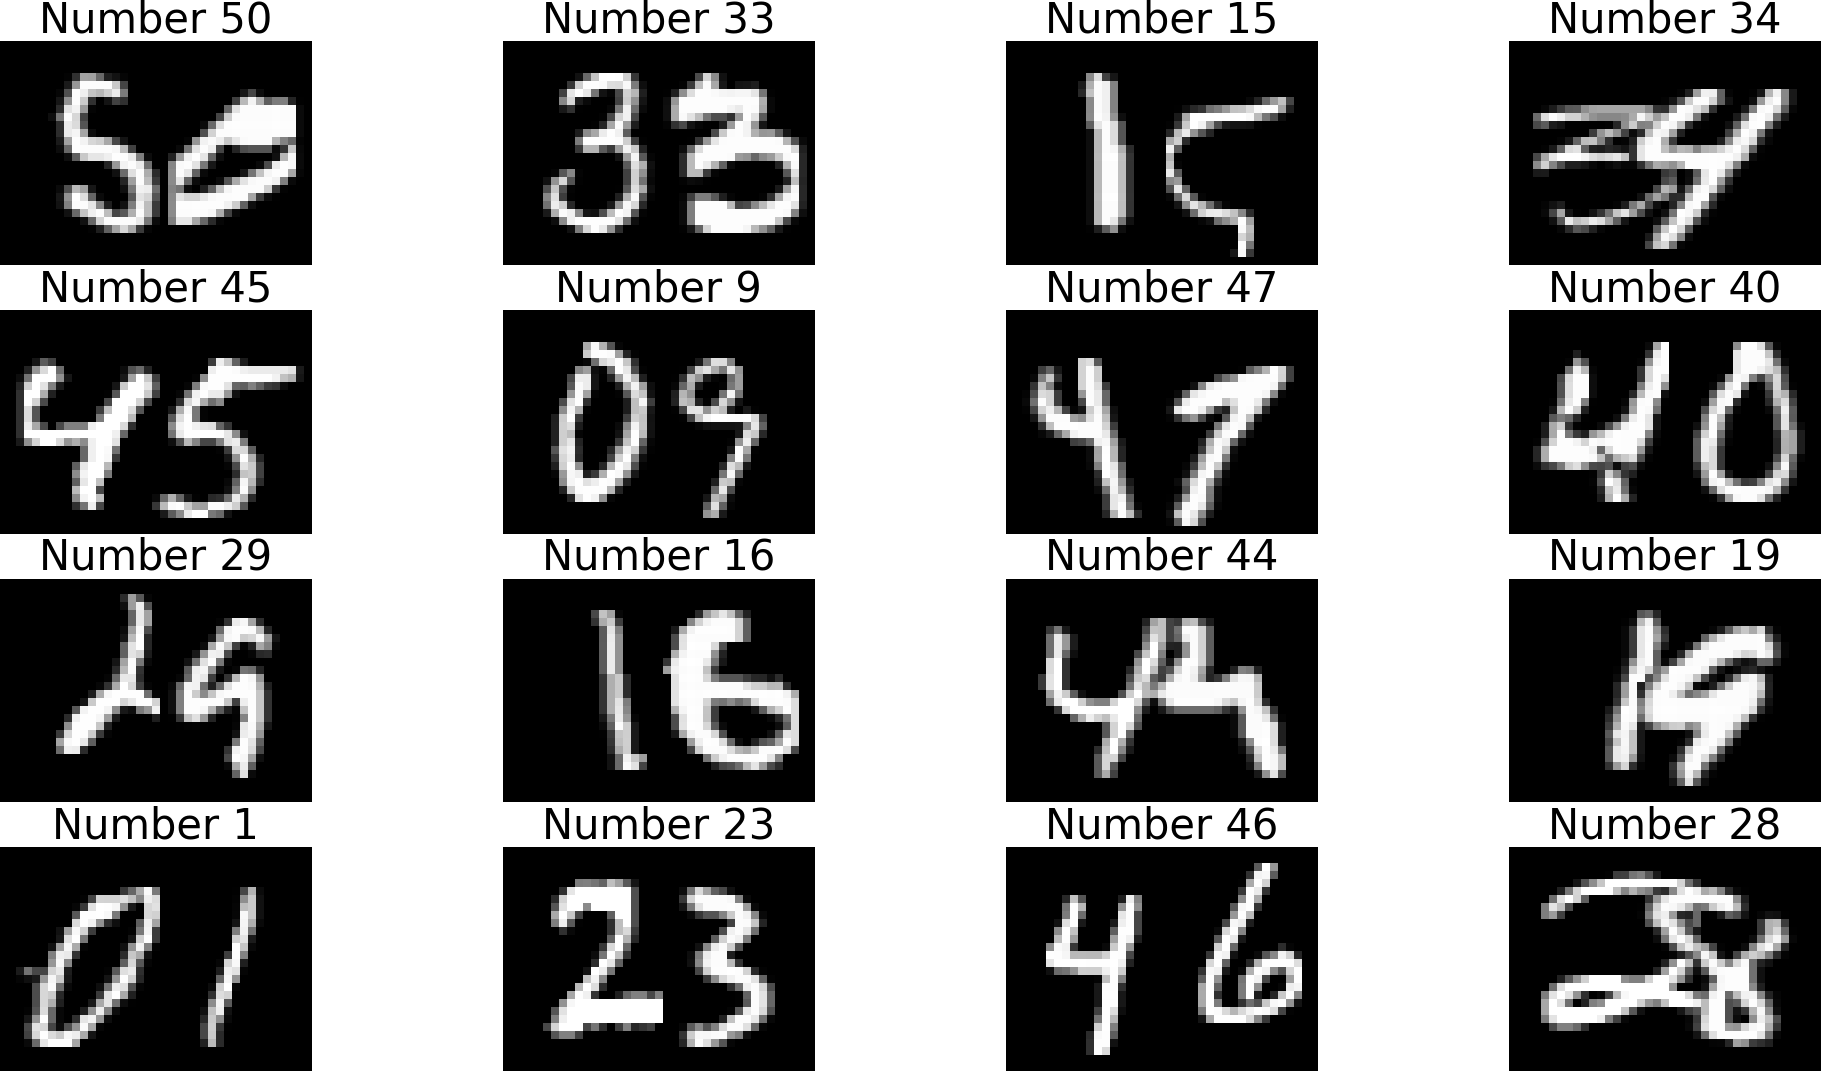
\includegraphics[width=3in]{sample.png}
\captionsetup{justification=centering}                                                                                                                                   
\caption{Sample of the first 16 unique samples}
\label{fig:sample}
\end{figure}

The data is already divided into training and test datasets. The first presents a non-uniform distribution of the classes,
as shown in Figure \ref{fig:datahist}. 
Many numbers have very low occurrencies, like 43 with 117 samples or 17 with 130 samples, against other like 11 with 3112 samples or 19 with $2\,890$ samples.
As a matter o fact the number of sample for each class in the training dataset has mean $\mu\simeq 1\,671$ and standard deviation $\sigma\simeq 1\,045$.

\begin{figure}[ht!]
\centering                                                                        
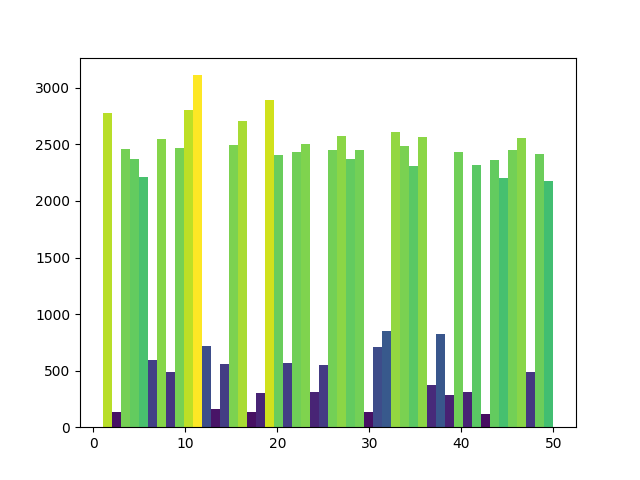
\includegraphics[width=3in]{datahist.png}
\captionsetup{justification=centering}                                                                                                                                   
\caption{Histogram of the frequency of samples in the dataset}
\label{fig:datahist}
\end{figure}


Along with the biases of the dataset, some number at first sight are difficult to interpret even to the human eye. For example,
Figure \ref{fig:unread} shows 6 difficult numbers to read: some have poorly defined lines and some have heavy overlappings. This may affect the
model's performance if those irregularities are more present in some classes.\par



\begin{figure}[ht!]
\centering                                                                        
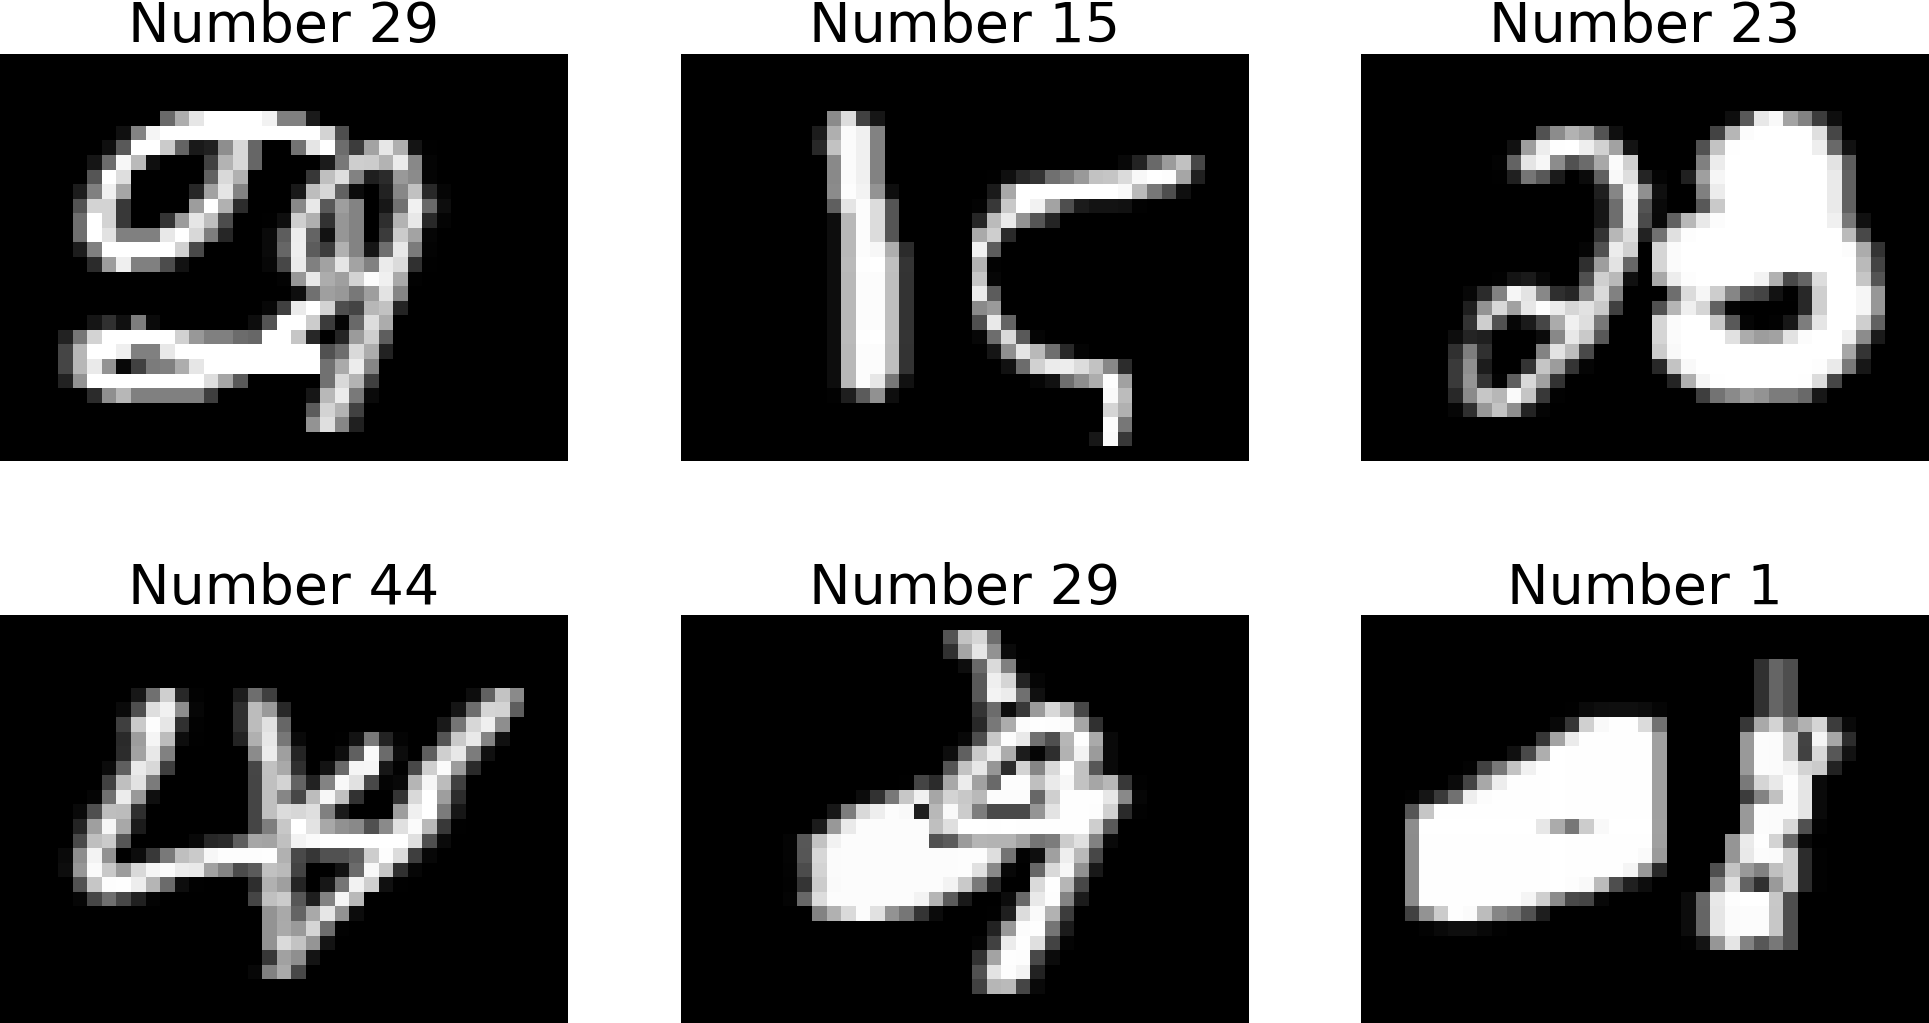
\includegraphics[width=2in]{unread.png}
\captionsetup{justification=centering}                                                                                                                                   
\caption{Numbers in the training set that are difficult to read even for a human being}
\label{fig:unread}
\end{figure}


Before training a FFNN using this images, encoded in $28\times39$ matrices with values from $0$ to $255$, we flattened them in
arrays $1\times1\,092$ and rescaled each value in the continuous interval $[0, 1]$. This encoding will be used in every section of this work: a flat array
better suits the input layer of a FFNN and small values increases the efficiency in the calculations
\footnote{Even if the final choices made for this work led to the usage of activation functions that were not affected by \emph{exploding gradient}, rescaling the values of the matrices helped the experimantations with other activation functions that were affected.}.


\subsection{Preparing the data}
As said in the section before, the dataset is divided into training and test samples. A validation subset is missing and thus
is retrieved from the training set: $20\%$ of the images are randomly used for validation instead of training (along with their labels). \par
About labels, we encoded them in one-hot vectors so that the $1$s are set in the index representing the numerical class. \par

Another, technical, issue is that \texttt{np\_utils.to\_categorical}, used to create the one-hot vectors, generated 51 classes instead of 50. That's because the function created as many classes as the highest value inside the input plus one: it took for granted that we were using a zero-based index. In order
to overcome this, without writing a similar function from scratch, we subracted 1 to each element of each vector inside the training and test label sets.
Obvisously that operation had been reverted when trying to predict the values.


\section{Unregularized FFNN}\label{sec:noreg}

The aim of this section is to describe a FFNN with less than $100\,000$ parameters that is able to classify
with high level of accuracy the numbers from the dataset without any regularization technique. 

\subsection{The network}
Because the number of parameters
are partially determined by the size of the input and output, we tested a FFNN with 2, 3, 4 and 5 hidden layers, but we found that 2-layers model
generalized better over a deeper (and less wide) model. Without entering in the details, the deepest model had 5 layers with 70 to 50 neurons each.\par 


We found a good spot with 80 neurons in the first layer and 50 in the second one, for a total of $96\,660$ parameters. 
Figure \ref{fig:noregffnn} shows the architecture of the network used in this section.






\begin{figure}[ht!]
\centering                                                                        
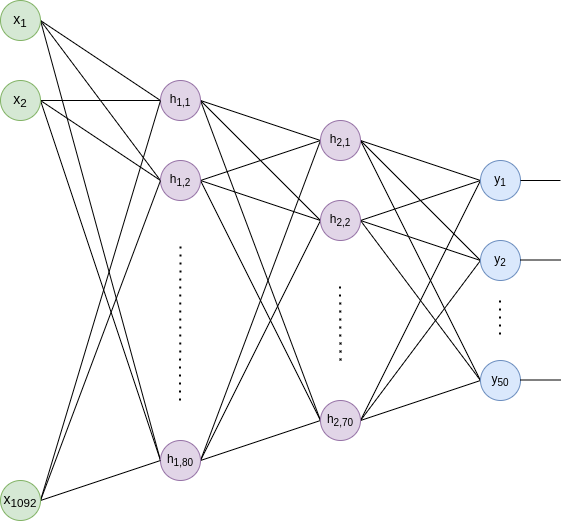
\includegraphics[width=2.5in]{noregffnn.png}
\captionsetup{justification=centering}                                                                                       
\caption{Architecture of the unregularized network}
\label{fig:noregffnn}
\end{figure}

Each hidden neuron used the \emph{Sigmoid} as activation function. We tried \emph{LeakyReLU} with $\alpha=0.01$ as well but resulting in a divergence in the model (the validation loss kept tp slighty grow after 15 epochs). The source was probably the explosion of the gradient caused by the function.  \par 
The output layer computes a \emph{Softmax}, which converts the input vector of real values to an output vector that can be interpreted as categorical probabilities.

\subsection{Training}
The choice of the optimizer was among \emph{SGD}, \emph{RMSProp} and
\emph{Adam}. This selection was influenced also by the initialization of the weights: 
\emph{SGD} performed well with \texttt{GlorotNormal} (also known as \emph{Xavier}) initializer but not as good as \emph{RMSProp} and
\emph{Adam} with \texttt{HeNormal}. \emph{SGD} with \texttt{HeNormal} resulted in a model that couldn't converge at all.

We tried all of them and chose \emph{Adam} with learning
rate of $10^{-3}$ , $\beta_1 = 0.9$ and $\beta_2 = 0.999$ because it seemed to
escape better from local minima, converging faster and giving
better accuracy. \par 
Because we are trying to find which images best suits in one of the 50 classes, the best loss function is the \emph{Categorical Cross-Entropy}.\par
The batch size of 256 gave the best results: 512 was another good choice but the convergence was slower and lower values of 256 performed worse; that might be
due to the fact that the model needed a good amount of variety of information before every update. But even using mini-batches of 8 the validation accuracy
reached $89\%$. When experimenting different batch sizes we always used powers of 2 in order to take advantage of the hardware parallelization.




\begin{figure}[ht!]
\centering                                                                        
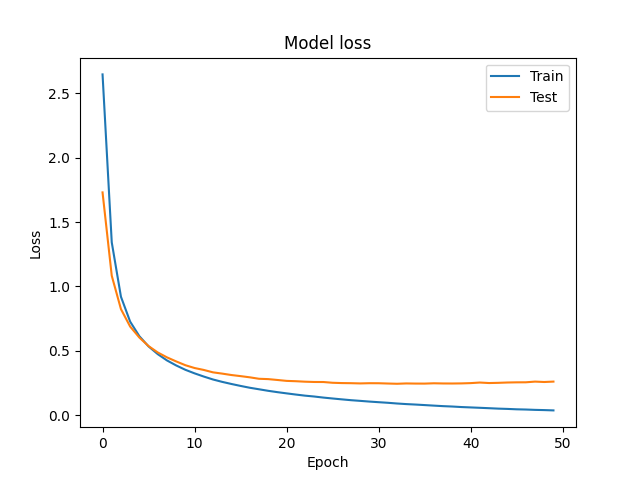
\includegraphics[width=3.5in]{../images/noreg/loss-sigmoid-categorical_crossentropy-Adam-50-256-final.png}
\captionsetup{justification=centering}                                                                                                                                   
\caption{Loss (unregularized)}
\label{fig:loss1}                                                                                                                                                           
\end{figure}


\begin{figure}[ht!]
\centering                                                                        
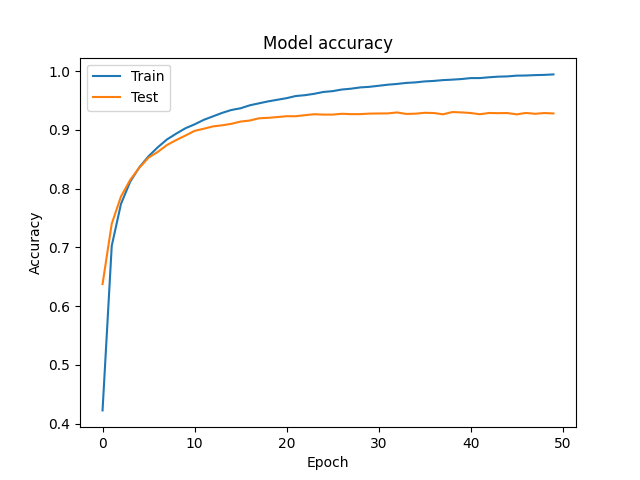
\includegraphics[width=3.5in]{../images/noreg/accuracy-sigmoid-categorical_crossentropy-Adam-50-256-final.png}
\captionsetup{justification=centering}                                                                                                                                   
\caption{Categorical accuracy (unregularized)}
\label{fig:acc1}                                                                                                                                          
\end{figure} 

We choose 50 as number of epochs in order to see the effects of missing regularization like \emph{early stopping}, 
even if the model reached an optimal state after 10 epochs. \par
As metric we used the \emph{categorical accuracy} because calculates the percentage of predicted values that match with true values for one-hot labels.
As shown in Figure \ref{fig:loss1} and \ref{fig:acc1} it is possible to see that the training validation reached $\sim100\%$ 
and the validation accuracy reached $91.5\%$ after 14 epochs and never got better. This means the model
overfitted too much and that would perform worse with samples it had never seen. \par


\subsection{Evaluation}

The categorical accuracy 
over the test set reached $89\%$ and can be analyzed with the help of the confusion matrix (Figure \ref{fig:noregcm}). 

\begin{figure}[ht!]
\centering                                                                        
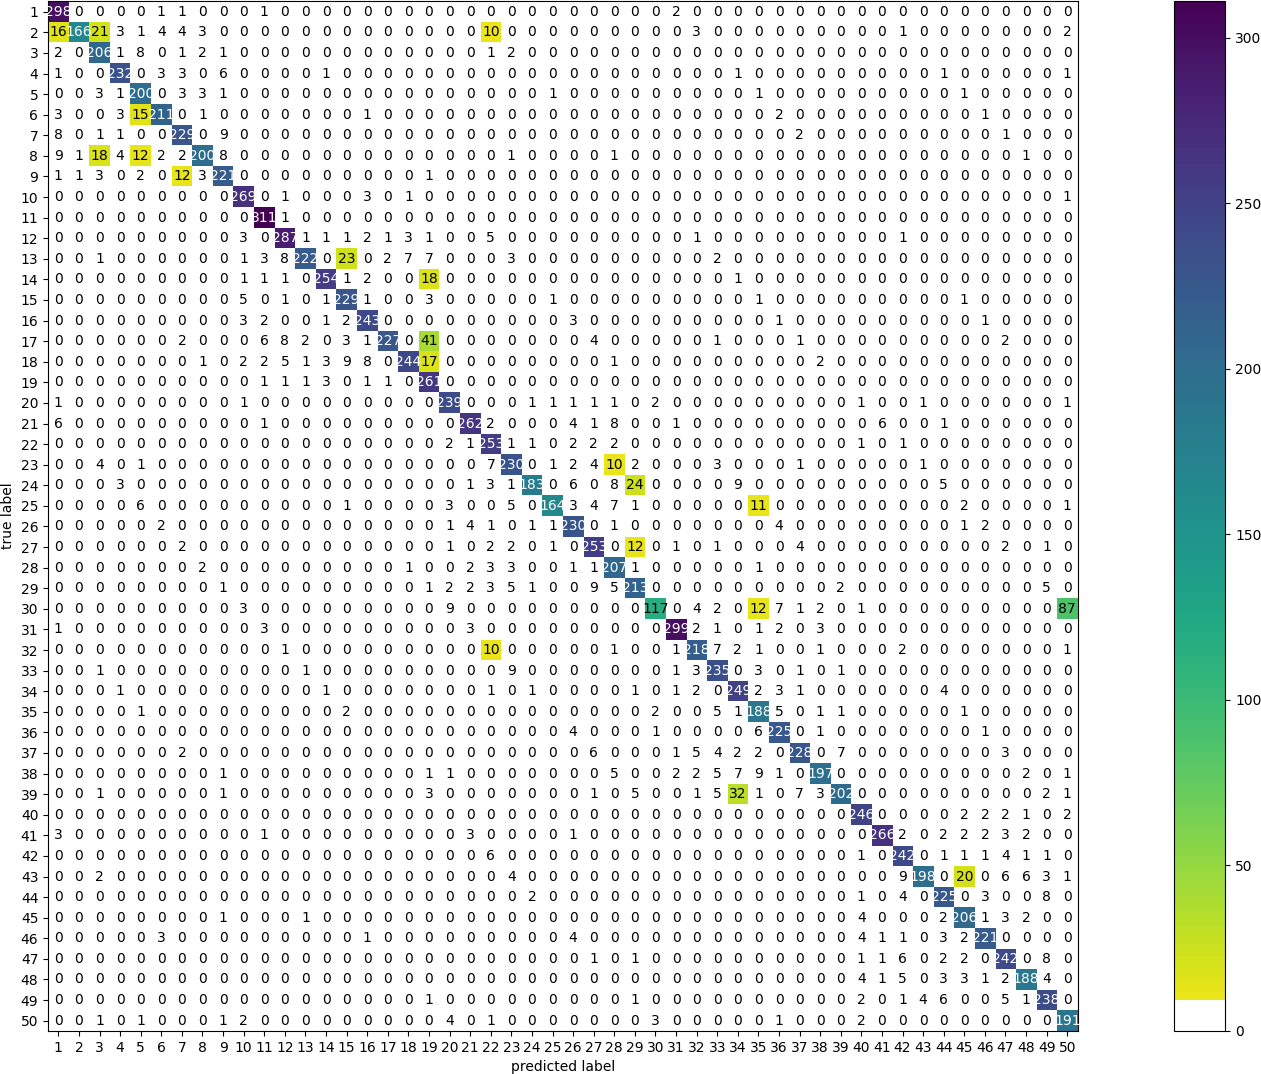
\includegraphics[width=3.5in]{noregcm.png}
\captionsetup{justification=centering}                                                                                 
\caption{Confusion matrix of the evaluation of the test set (unregularized network)}
\label{fig:noregcm}                                                                                                                        
\end{figure}
The confusion matrix uses a custom colormap (\emph{viridis} but with the first 10 values set to 0) so that was easier
to hide negligible errors (in this case less than 10 mismatches) in such a large matrix. It is noticeable that the model confuses number 50 with 30,
19 with 17, 34 with 39 and others. These errors are not only due to the similarity between their digits, but because
these are the classes with less elements in the training set. So with no surprise the unbalances inside the training set played an
important role.\par





\section{Regularized FFNN}
The aim of this section is to describe a FFNN with less than $100\,000$ parameters that is able to classify
with high level of accuracy the digits from the dataset with one or more regularization technique. 

\subsection{The network}
We wanted to keep the network as simiar as possible to the one described in Section \ref{sec:noreg} in order to better measure the effects of regularization.
For this reason we used the very same architecture as base (2 layers, 80 and 70 neurons).
The only thing that changed was the activation functions: we switched \emph{Sigmoid} with \emph{LeakyReLU}s because the first outperformed the second. Probably the effect of \emph{exploding gradient} was restrained by the regularization and a \emph{Sigmoid}-based model suffered too much the underfitting.


\subsection{Regularization techniques}\label{sec:reg}
In this section we describe the techiques tested, used or discarded to achieve a lower level of underfitting and secondary to reach a better level of accuracy.

\subsubsection{Data augmentation}
The first attempt of undirect regularization involved filling the gap between the classes by generating new samples for the less populated classes. The procedure, described in Algorithm \ref{alg:aug}, generates for each class as many samples as there are in the percentage $p$ of the difference with the most populated class.
By choosing $p=0.1$ each class diminuished the gap with the major class by $10\%$. \par
Three techniques were taken in account: \emph{adding noise}, \emph{image shifting} and \emph{image rotation}. The first added a gaussian noise $\mathcal{N}(0, \frac{1}{2})$, the second randomly shifted the image long the 2 axis by 2 pixels (2 positions in the matrix) in both directions and the third rotated the image by a random angle bewteen $-20^{\circ}$ and $20^{\circ}$. \par
None of the above helped the network: the level of accuracy dropped to $86\%$ and the loss was very high when applying noise ($\geq 0.6$). Image roation alone is the only one that didn't make the accuracy worse. For these reasons data augmentation was discarded even if theoretically speaking filling the gap between samples made sense. Probably the model already recognized the single features of those samples so that adding similar samples just increased redundancy.

\begin{algorithm}[h]
\SetAlgoLined
\KwData{$X$ training samples, $Y$ training labels, $p \in [0, 1]$}
\KwResult{$X$ augmented, $Y$ augmented }
$l=|Y|$\;
$C \gets \{\}$\;
\For{$i \gets 1$ \textbf{to} $l$}{
\eIf{$Y_i \in C$}{
$C_i \gets C_i + 1$\;
}{
$C_i \gets 1$\;
}
}


$m \gets \max_k C_k$\;

\For{$(k,v) \in C$}{
$S = \{e \in X : e = k\}$\;
$g \gets \left \lfloor (m-v) \cdot p \right \rfloor$\;
\For{$i \gets 1$ \textbf{to} $g$}{
$x \gets augment(S_{random})$\;
$\text{append } x \text{ to } X$\;
$\text{append } k \text{ to } Y$\;
}
}
\Return $shuffle(X, y)$\;

\caption{Data augmentation algorithm}\label{alg:aug}
\end{algorithm}


\subsubsection{L1 and L2}
\emph{L1} and \emph{L2} are typical techniques used to reduce the overfitting of the model by settings penalties in the coeffiecients. We tried first \emph{L1}, but even with low regularization factors (from $10^{-3}$ to $10^{-5}$) the model underfitted too much. \emph{L2} with a regularization factor of $10^{-5}$ performed better, similar to a a regularization factor of $10^{-4}$ and a learning rate 10 times higher ($10^{-2}$), but was outperformed in accuracy by a model not implementing it.

\subsubsection{Dropout}
\emph{Dropout} turned out to be a good choice: it decreased the overfitting without losing too much accuracy. We chose a drop out probability for each layer of $10\%$ because the network wasn't too big and higher probabilities gave worse results. This strategy helped the network to ignore certain features of the images or the $0s$ of the matrices (black spaces). A representation of the network can be found in Figure \ref{fig:regffnn}. 

\begin{figure}[ht!]
\centering                                                                        
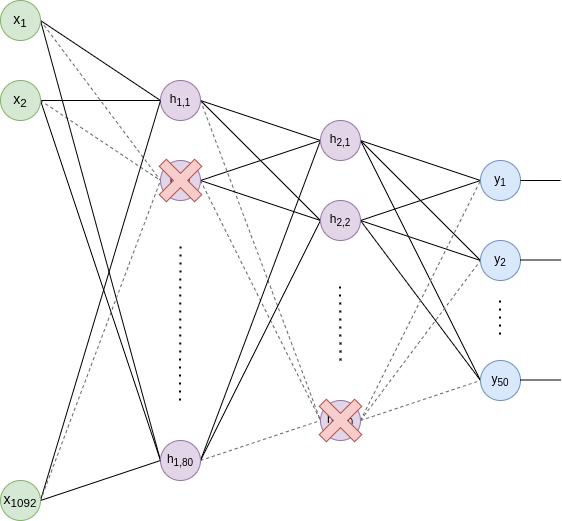
\includegraphics[width=2.5in]{regffnn.png}
\captionsetup{justification=centering}                                                                                                           
\caption{Architecture of the network with dropout}
\label{fig:regffnn}
\end{figure}

\subsubsection{Early stopping}
Another game changer was the application of \emph{early stopping} over the validation process, with a patience factor of 10 epochs and a minimum $\delta = 0.05$. This greately reduced the overfitting and because the model converged after 15-20 epochs we restored the weights to the last best snapshot ($20^{\text{th}}$ epoch).




\subsection{Training}
The optimizer used was \emph{Adam} with a learning rate of $10^{-3}$ in conjuction with $\texttt{HeNormal}$ initializer. We used 50 epochs and batches of 256 elements 
not only to replicate the methodologies used with the unregularized model, but because outperformed other configurations. This means that the addition of dropout hasn't changed the quantity of information needed by the model before an update.



\begin{figure}[ht!]
\centering                                                                        
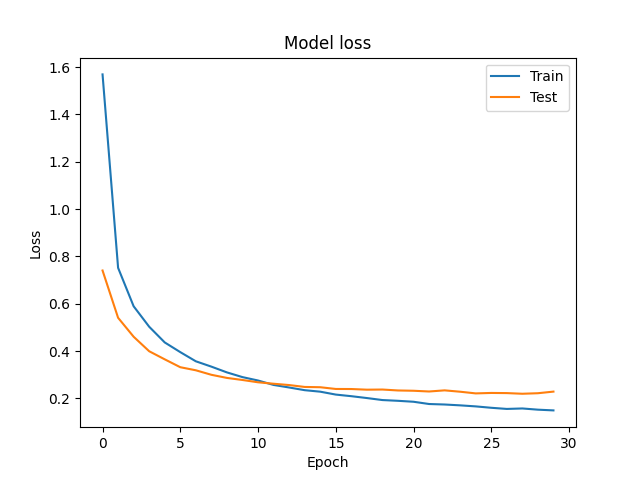
\includegraphics[width=3.5in]{../images/reg/loss-LeakyReLU-NoneType-categorical_crossentropy-Adam-50-256-0.1-final.png}
\captionsetup{justification=centering}                                                                                                                              
\caption{Loss (unregularized)}
\label{fig:loss2}                                                                                                                                         
\end{figure}


\begin{figure}[ht!]
\centering                                                                        
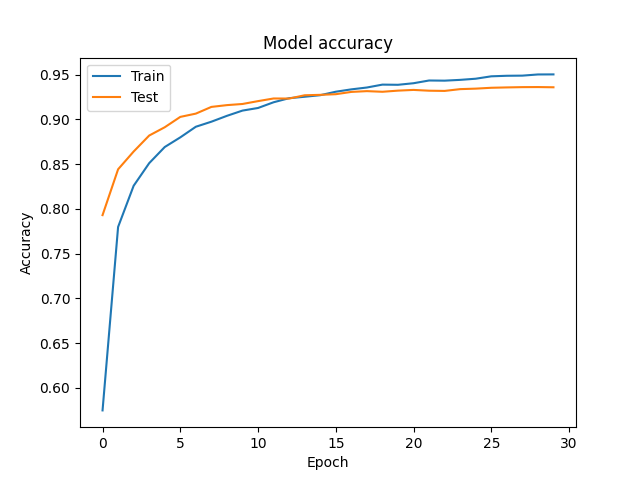
\includegraphics[width=3.5in]{../images/reg/accuracy-LeakyReLU-NoneType-categorical_crossentropy-Adam-50-256-0.1-final.png}
\captionsetup{justification=centering}                                                                                                                            
\caption{Categorical accuracy (unregularized)}
\label{fig:acc2}                                                                                                                                          
\end{figure} 


\subsection{Evaluation}

The validation accuracy reached $93\%$ ($+1.5\%$ over the unregularized model) but with a training accuracy of $94\%$: this means the model had less memorized the dataset in favor of a better generalization. The test accuracy reached $92\%$ ($+3\%$) and this proved that the model implementing regularization techniques 
had a higher capabilities to generalize the problem. \par
The confusion matrix in Figure \ref{fig:regcm} shows the improvements made from the previous model: there are still some mismatches between predicted and true labels, but they have lower intensity \emph{i.e.} there are less cases where the $50$ is confused with $30$ ($-28\%$) or $19$ with $17$ ($-70\%$).\par
The regularization definetely changed the network performances without changing the architecture per se.

\begin{figure}[ht!]
\centering                                                                        
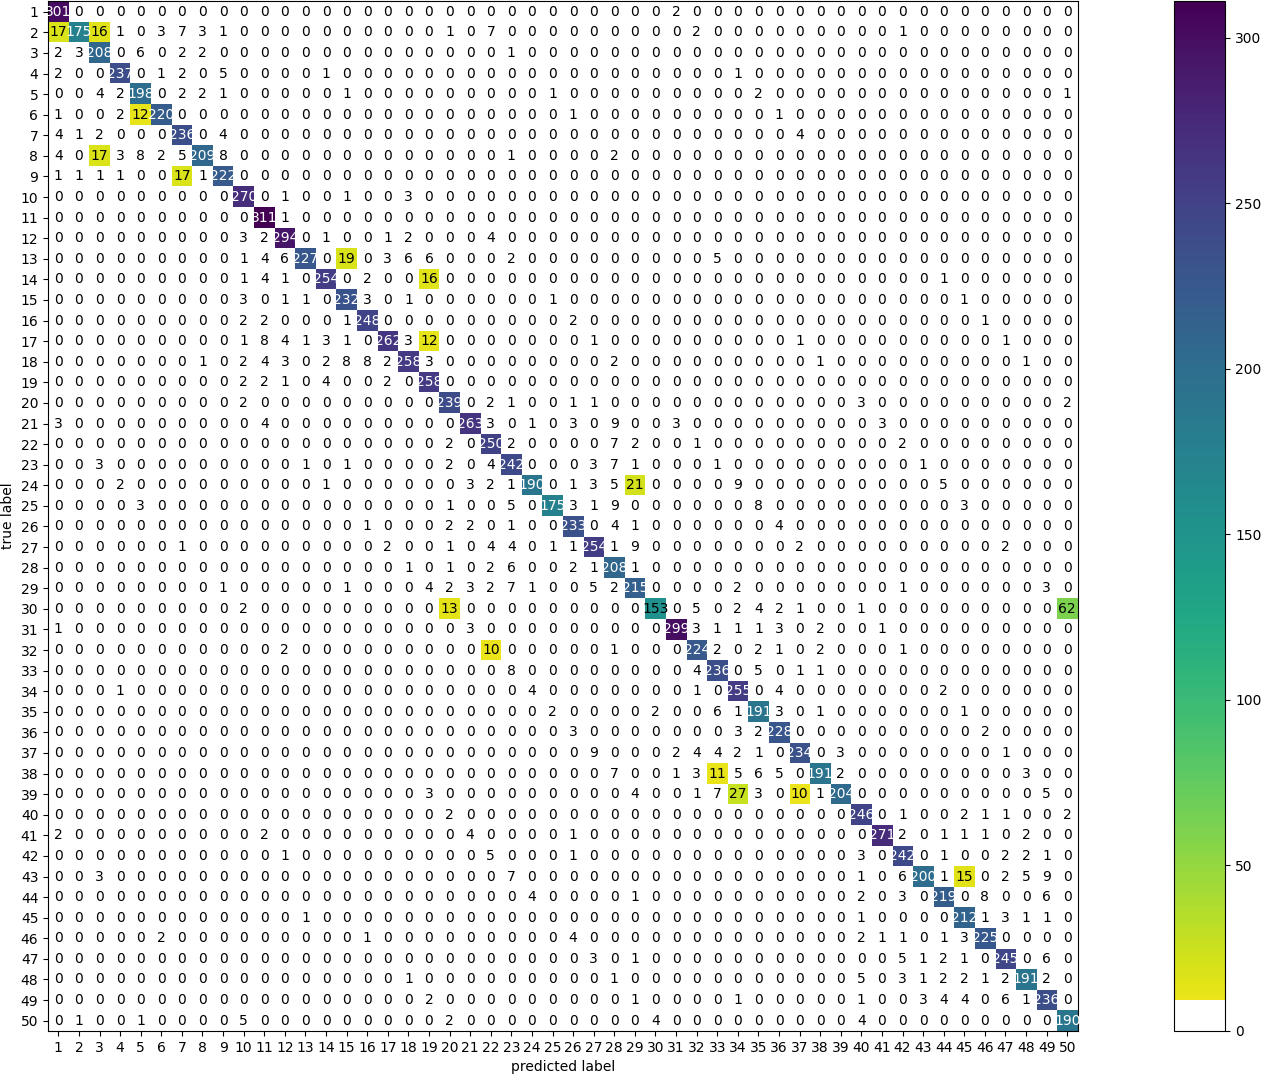
\includegraphics[width=3.5in]{regcm.png}
\captionsetup{justification=centering}
\caption{Confusion matrix of the evaluation of the test set (regularized network)}
\label{fig:regcm}
\end{figure}


\section{Autoencoding}
In this section we show how to build an autoencoder that compresses the knowledge of the original input and that reconstructs the input starting from the compessed (encoded) version.
\subsection{The nerwork}\label{sec:autonet}
Before deciding the compression rate, we describe here the foundamentals of the autoencoder's architecture. The input, like in the previous cases, is represented by a flatten version of the images, that is a $1\times1\,092$ array. Because it is an autoencoder, the same goes for the output. We chose 2 hidden layers for the encoder and 3 for decoder; we used this "unbalance" because it easy for the network to compress information but harder to decompress them. So the decoding part uses a more complex model.\par
The compression factor that defines the lenght of the encoding had been decided with a benchmark: we trained 10 networks with different compression factors (from 20 to 30) and analyzed their mean squared errors (\emph{MSE}) when trying to reproduce the input. Figure \ref{fig:multiacc} and \ref{fig:mse} demonstrates that the best compression factor was $28$, that is having an encoded layer formed by 39 neurons. This result depends more on the architecture of the network rather than the problem itsel, but it is noticeable and not so expected that the plot in Figure \ref{fig:mse} does not represent a monotonic function nor an increasing function.\par



\begin{figure}[ht!]
\centering                                                                        
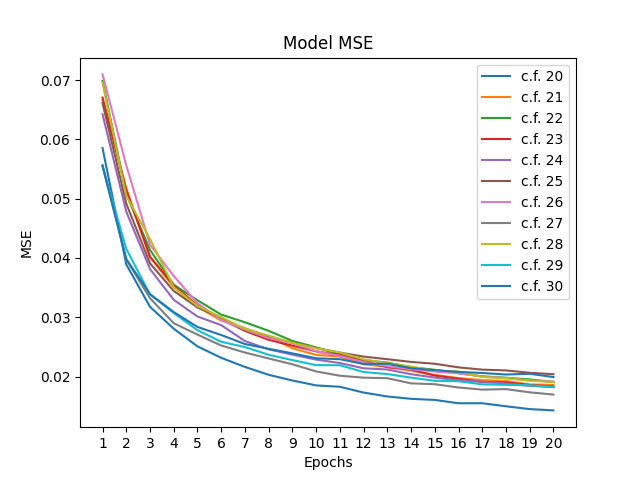
\includegraphics[width=3.5in]{multiacc.png}
\captionsetup{justification=centering}                                                                                         
\caption{\emph{MSE} vs. number of epochs with multiple compression factors}
\label{fig:multiacc}
\end{figure}

\begin{figure}[ht!]
\centering                                                                        
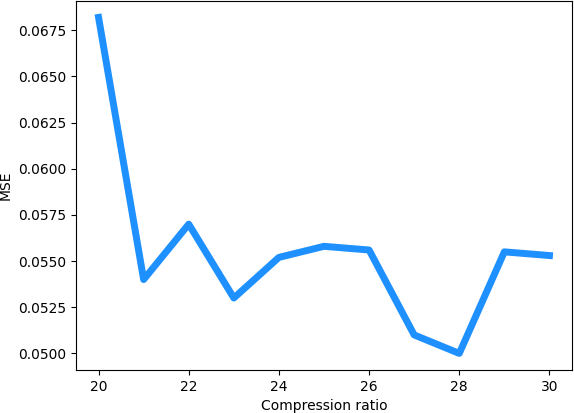
\includegraphics[width=2.5in]{mse.png}
\captionsetup{justification=centering}                                                                                                                              
\caption{\emph{MSE} with different compression factors}
\label{fig:mse}                                                                                                                                         
\end{figure}


Figure \ref{fig:auto} shows the final architecuture of the autoencoder: $1\,092$ neurons for input, 256 and 128 for encoding, 39 for storing the compressed knowledge, 128, 256 and 512 for decompression and $1\,092$ for output.\par
All the layers used \texttt{LeakyReLU} with $\alpha=0.01$ as activation function. The output layer used a \emph{Sigmoid} that better represents values between 0 and 1.

\subsection{Training}\label{sec:autotrain}
For the training phase we used \emph{Adam} but with \emph{binary crossentropy} loss function. \emph{Binary crossentropy}, based on the logarithmic operation, 
better avoids the effects present in the \emph{Sigmoid} function, that is based on the exponential function.

\begin{figure}[ht!]
\centering                                                                        
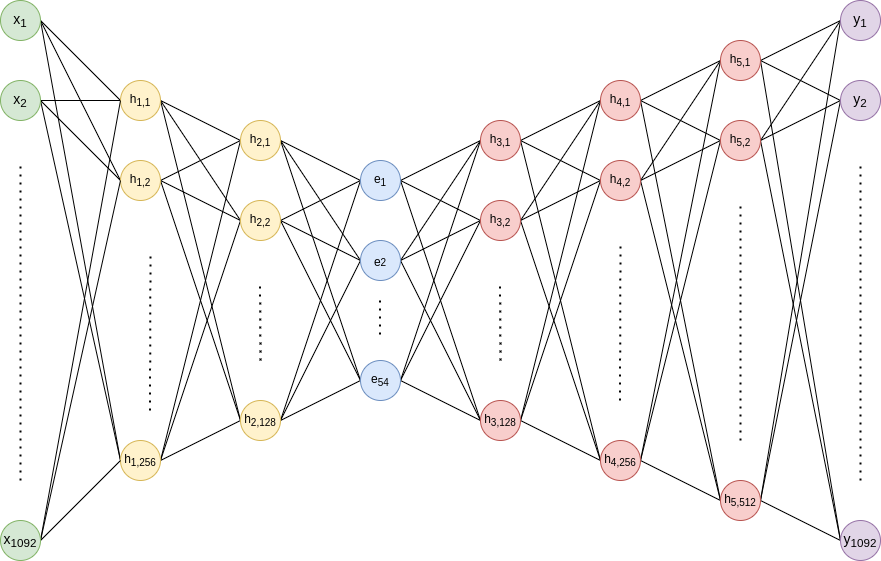
\includegraphics[width=3.5in]{auto.png}
\captionsetup{justification=centering}
\caption{Final architecture of the autoencoder: in green the input, in yellow the encoders, in blue the latent layer, in red the decoders and in purple the output}
\label{fig:auto}
\end{figure}

\subsection{Evaluation}
The best way to evaluate the autoencoder, other than plotting the loss and the \emph{MSE}, is to visualize the results (Figure \ref{fig:reproduce}). In the first row
there are 10 samples from the test set while in the second row the output of the autoencoder. The similarity between the two sequences is quite high, but we
can notice that the second row presented a certain level of blurriness. This is caused by the data lost during the encoding and the fact that the model didn't  converged to a global minimum (lossless compression).


\begin{figure}[ht!]
\centering                                                                        
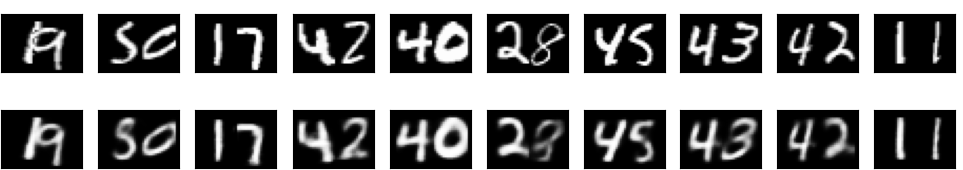
\includegraphics[width=3.5in]{reproduce.png}
\captionsetup{justification=centering}
\caption{First row: original test data. Second row: the same input but reproduced by the autoencoder.}
\label{fig:reproduce}
\end{figure}

\subsection{Generation}
In order to generate random new samples, we trained the autoencoder as previously done in section \ref{sec:autotrain} and used only the second part of the architecture, that is 
from the encoded layer to the output (Figure \ref{fig:generator})


\begin{figure}[ht!]
\centering                                                                        
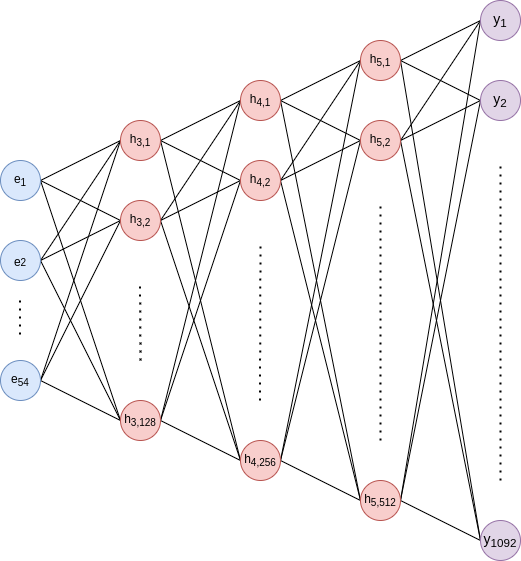
\includegraphics[width=2.5in]{generator.png}
\captionsetup{justification=centering}
\caption{Architecture of the generator: the input and encoding layers are removed from the Autoencoder}
\label{fig:generator}
\end{figure}

We fed the model with random numbers with two different distributions: the first is a uniform distribution $U(0, 1)$ and the second a custom one we describe later.\par
The random input with uniform distribution gave the results shown in Figure \ref{fig:unif}

\begin{figure}[ht!]
\centering                                                                        
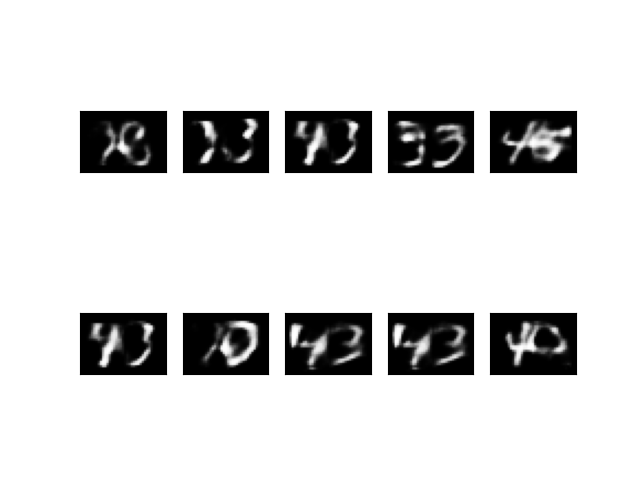
\includegraphics[width=2.5in]{unif.png}
\captionsetup{justification=centering}
\caption{New samples generated from a uniform distribution}
\label{fig:unif}
\end{figure}

Some digits are distinguishable (like 38, 33, 40, 43 and 45) but they are blurry, lowly defined and redundant (many $33$ and $43$).

\begin{figure}[ht!]
\centering                                                                        
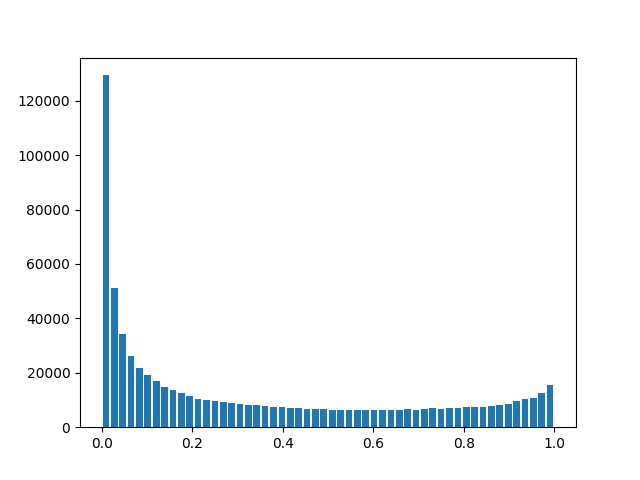
\includegraphics[width=3.5in]{enco.png}
\captionsetup{justification=centering}
\caption{Means and deviations standard of each column of the encodings generated over the training set}
\label{fig:enco}
\end{figure}

Because results were not exhaustive, we andalyzed the distribution in the encoded layer after having fed the network with the entire
test set. Figure \ref{fig:enco} demonstrate that the distribution is far from being uniform.


So we implemented a custom distribution that tried to emulate the real distribution
present in the encoded layer after feeding the model with entire test set. Algorithm \ref{alg:ran} describes the procedure.

\begin{algorithm}[h]
\SetAlgoLined
\KwData{$P \textnormal{ matrix of predictions over } X_{test}$, $n \in \mathbb{N} \textnormal{ number of encodings}$}
\KwResult{\emph{$E \textnormal{ matrix of random } $n$ \textnormal{ encodings}$}}

$E \gets \mathcal{M}(n \times 39)$\;
\For{$i \gets 1$ \textbf{to} $n$}{

\For{$j \gets 1$ \textbf{to} $39$}{

$column \gets P_{*,j}$\;
$m \gets \mu(column)$\;
$s \gets \sigma(column)$\;
$E_{i,j} \gets random(\mathcal{N}(m, s))$
}

}



\Return $E$\;

\caption{Custom distribution}\label{alg:ran}
\end{algorithm}

The procedure calculates a new matrix of encodings, generated by a normal distribution $\mathcal{N}(\mu, \sigma)$ on each column, where $\mu$ and $\sigma$ are calculated on the same column of the matrix of encodings. Since the first dimension describes different sequences, what is important is to maintain the distribution
of each column. That's because the weights in the encoding layer (like in any other) cannot be permutated without affecting the final result of the model. That's why we emulated the distribution by column, assuming that the values are normally distributed (which is probably not, but this should require more time into investigation). 


\begin{figure}[ht!]
\centering                                                                        
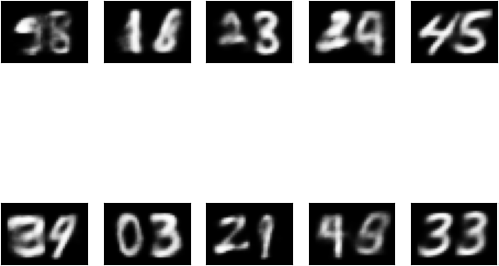
\includegraphics[width=2.5in]{gen.png}
\captionsetup{justification=centering}
\caption{}
\label{fig:gen}
\end{figure}

Figure \ref{fig:gen} shows the results, which are way better than the ones generated with a uniform distribution. We can find sharper shapes, a little bit of more
diversity in the digits (although there are many $3$s). What is very interesting is the appearance of a $98$, even if the network has been trained on numbers between $1$ and $50$. This suggests that the order of the weights matters but it doesn't describe the order of the digits; that is quite predictable since the layers are densely-connected and every neuron can affect any other neuron of the next layer.


\section{Combination of the latent representation with SVMs}
In this section we built an hybrid architecture with FFNN and a non-linear SVM. The input flows into the encoder described in section \ref{sec:autonet} in order to generate a latent representation. This representation is used to feed a SVM that solves the classification task. 
\subsection{Architecture}
The architecture is shown in Figure \ref{fig:svm}. We used the same encoder with the same activation functions and number of neurons per layers. On the other side,
we had to calculate the optimal cost parameter of the SVM. This parameter decided the size of the margin hyperplane (the higher the cost the smaller the margin) and thus it made the model penalize less or more the samples inside the margin. \par

\begin{figure}[ht!]
\centering                                                                        
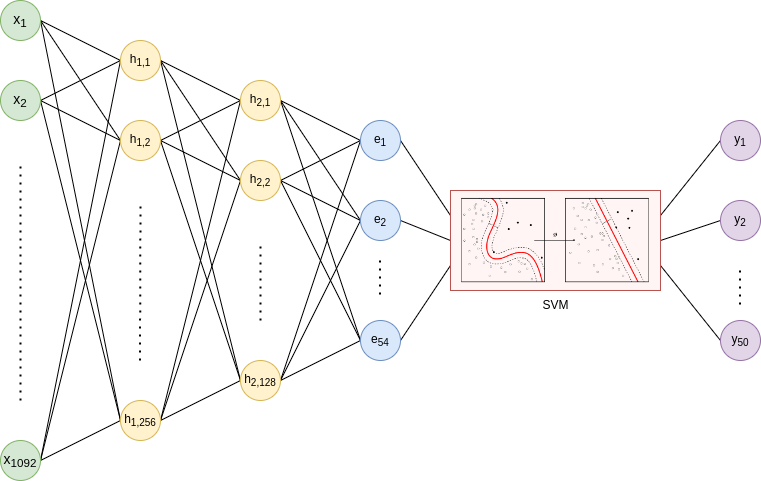
\includegraphics[width=3.5in]{svm.png}
\captionsetup{justification=centering}                                                                                       
\caption{Architecture of the encoder that feeds the SVM}
\label{fig:svm}
\end{figure}


In order to decide the cost parameter, we trained the SVM with multiple costs in a logarithmic scale: from $10^{-4}$, to $10^{4}$. We measured the accuracy both with training and test set to evaluate the overfitting of the SVM. To speedup the process we used only 1000 samples per training since SVM training time grows as $O(f(C,  d \cdot |X^{train}|^2))$ where $f$ is some increasing function, $C$ is the cost parameter and $d$ is the number of features in the training set $X^{train}$.\par
The output of this procedure is shown in  Figure \ref{fig:svmacc}. We noticed that the model starts to overfit with cost $C \geq 10$, so we tested the interval $1 \leq C \leq 10$ and the model scored a maximum accuracy of $84,8\%$ with $C=10$ over the entire test set. 


\begin{figure}[ht!]
\centering                                                                        
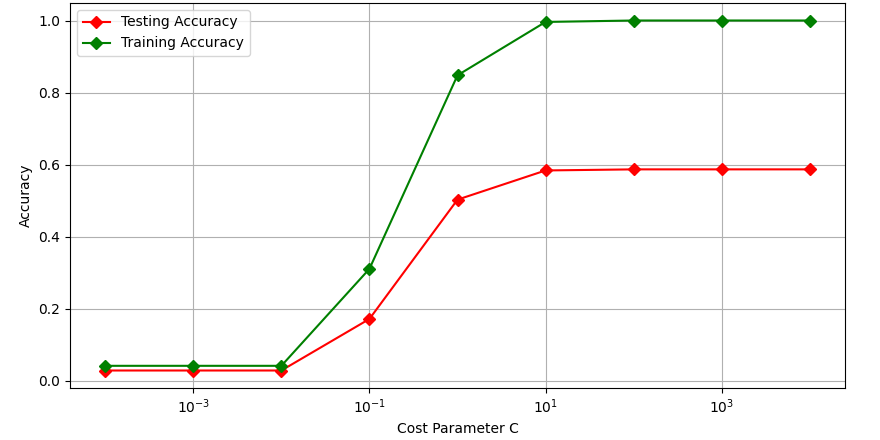
\includegraphics[width=3.5in]{svmacc.png}
\captionsetup{justification=centering}                                                                                       
\caption{Accuracy vs. cost parameter $C$ (logarithmic scale)}
\label{fig:svmacc}
\end{figure}

This test produced the confusion matrix in Figure \ref{fig:c10}. We noticed that the model is less accurate than the unregularized and regularized models and it still maintains their same weaknesses: the less populated classes suffered of higher level of confusion $i.e.$ it confused numbers 50 with 30, 19 with 17 and 34 with 39.


\begin{figure}[ht!]
\centering                                                                        
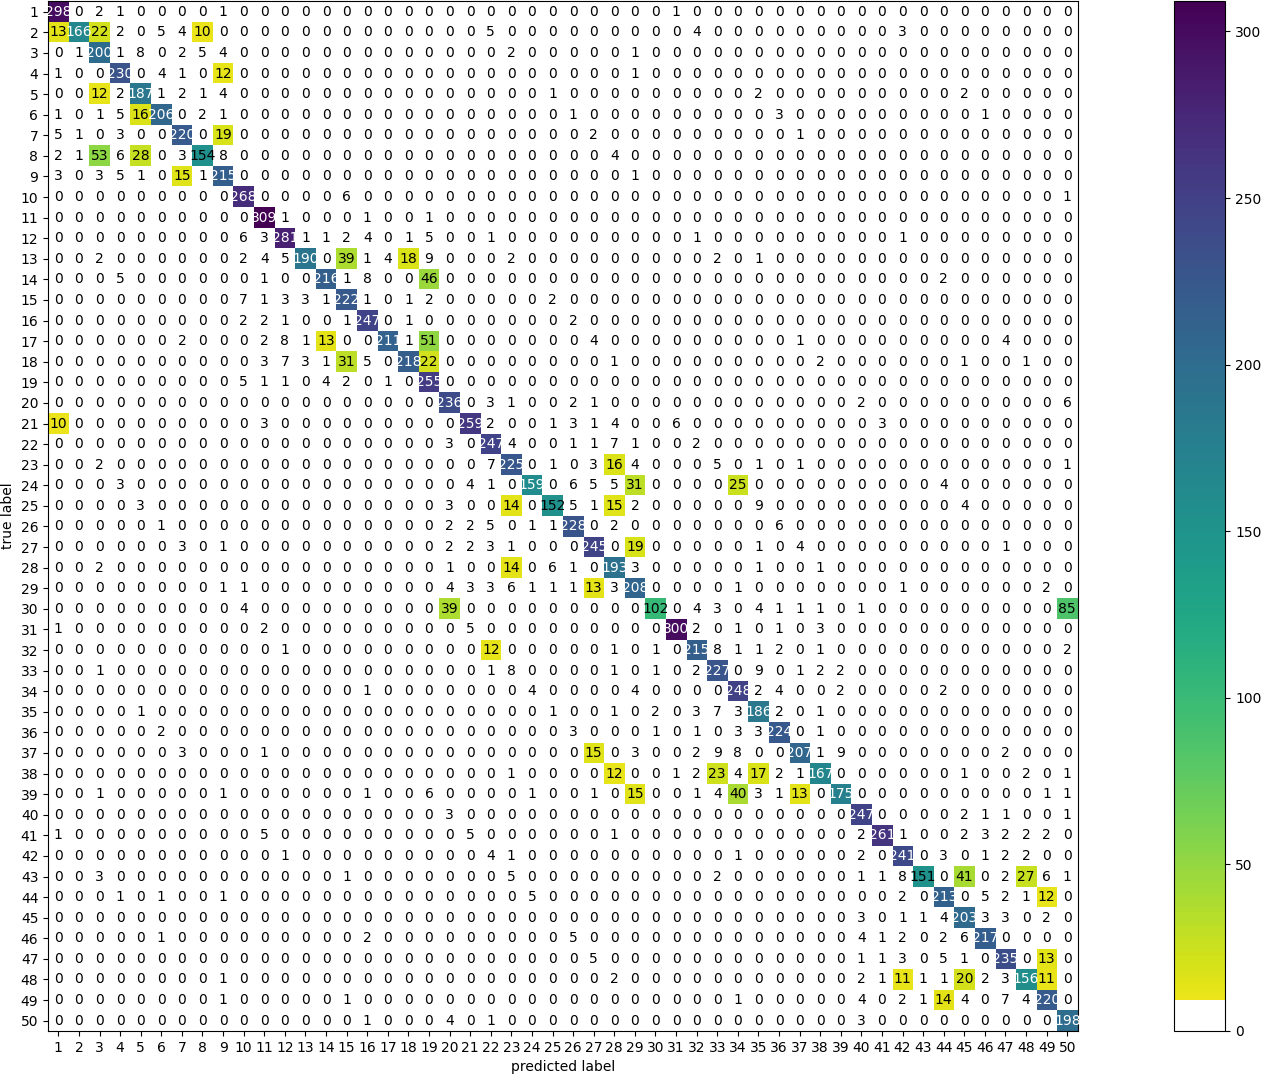
\includegraphics[width=3.5in]{c10.png}
\captionsetup{justification=centering}                                                                                       
\caption{Confusion matrix of the hybrid model with $C=10$}
\label{fig:c10}
\end{figure}

Even if the results is not as good as the regularized model's ones, the experiment was not a complete failure. We demonstrate that is possible to train hybrid ML models with good results; also it doesn't mean that a better integration between a FFNN and other classical ML models doesn't exist. This case study covered only non-linear SVMs.

\section{Implementations}
The training of the unregularized model can be started with \texttt{noreg-training.py}. It generates the needed images for the project in \texttt{./images/noreg/}
a model checkpoint (hdf5 file) in in \texttt{./noreg}. The validation can be performend with \texttt{noreg-eval.py}.\par
The training of the regularized model can be started with \texttt{reg-training.py}. It generates the needed images for the project in \texttt{./images/reg/}
a model checkpoint (hdf5 file) in in \texttt{./reg}. The validation can be performend with \texttt{reg-eval.py}.\par
Training, reconstruction and generation of new samples via autoencoder can be started with \texttt{generate.py} \par
Training and validation of the hybrid model can be started with \texttt{svm.py}


\section{Conclusions}
In this work we trained a FFNN on a custom MNIST dataset without any regularization technique and compared the same FFNN with dropout and early stopping techniques. We found out that the second one performed better during both training and test phase; regularization techniques are a powerfull tool that
prevents overfitting even without changing the overall architecture. We tried also data augmentation and \emph{L1}/\emph{L2} penalizations but with worse results. \par
The constraint of $100\,000$ parameters played an important role in the decisions made; without it other form of regularization would have shined and outperformed the unregularized model with a larger gap. \par 
We build an autoencoder and used its parts to generate new random samples and attach it to a SVM to classify the samples. 
In the first case we discovered that the generation of new samples cannot be accomplished by using any random distribution and that the model was able to produce meaningful images whose class was not part of the training dataset; in the second case we demonstrated that hybrid architectures can give good results, although the FFNN with regularization gave the best results. 


\end{document}









